\documentclass{article}
\usepackage{amsmath}
\usepackage{titlesec}
% \usepackage[mathletters]{ucs}
\usepackage{mathtools} %for \abs{x}
\usepackage[warnings-off={mathtools-colon,mathtools-overbracket}]{unicode-math}
% \setmainfont{TeX Gyre Schola}
% \setmathfont{TeX Gyre Schola Math}
% \usepackage[utf8x]{inputenc}
\usepackage{fontenc}
\usepackage[margin=1.5in]{geometry}
\usepackage{enumerate}
\newtheorem{theorem}{Theorem}
\usepackage[dvipsnames]{xcolor}
\usepackage{pgfplots}
\pgfplotsset{compat=1.18}
\setlength{\parindent}{0cm}
\usepackage{graphics}
\usepackage{graphicx} % Required for including images
\usepackage{subcaption}
\usepackage{bigintcalc}
\usepackage{pythonhighlight} %for pythonkode \begin{python}   \end{python}
\usepackage{appendix}
\usepackage{arydshln}
\usepackage{physics}
\usepackage{booktabs} 
\usepackage{adjustbox}
\usepackage{mdframed}
\usepackage{relsize}
\usepackage{physics}
\usepackage[thinc]{esdiff}
\usepackage{esint}  %for lukket-linje-integral
\usepackage{xfrac} %for sfrac
\usepackage[colorlinks=true,linktoc=page]{hyperref} %for linker, må ha med hypersetup
\usepackage[noabbrev, nameinlink]{cleveref} % to be loaded after hyperref
% \usepackage{amssymb} %\mathbb{R} for reelle tall, \mathcal{B} for "matte"-font
\usepackage{listings} %for kode/lstlisting
\usepackage{verbatim}
\usepackage{graphicx,wrapfig,lipsum,caption} %for wrapping av bilder
\usepackage[english]{babel}
\usepackage{cancel}
% \usepackage{alphabeta}
\usepackage{mhchem} % for atom notasjon
% \definecolor{codegreen}{rgb}{0,0.6,0}
% \definecolor{codegray}{rgb}{0.5,0.5,0.5}
% \definecolor{codepurple}{rgb}{0.58,0,0.82}
% \definecolor{backcolour}{rgb}{0.95,0.95,0.92}
% \lstdefinestyle{mystyle}{
%     backgroundcolor=\color{backcolour},   
%     commentstyle=\color{codegreen},
%     keywordstyle=\color{magenta},
%     numberstyle=\tiny\color{codegray},
%     stringstyle=\color{codepurple},
%     basicstyle=\ttfamily\footnotesize,
%     breakatwhitespace=false,         
%     breaklines=true,                 
%     captionpos=b,                    
%     keepspaces=true,                 
%     numbers=left,                    
%     numbersep=5pt,                  
%     showspaces=false,                
%     showstringspaces=false,
%     showtabs=false,                  
%     tabsize=2
% }

% \lstset{style=mystyle}

\author{Oskar Idland}
\title{Problem Set 8}
\date{}
\begin{document}
% \tableofcontents
\maketitle
\newpage

\subsection*{Problem 1 (6.1)}
\begin{mdframed}
Define charged and neutral current reactions in weak interactions and give an example of each in symbol form. How do they differ in respect of conservation of the strangeness quantum number? Why does observation of the process $ν_{μ} + e^{-} →  ν_{μ} +  + e^{-}$ constitute unambiguous evidence for weak neutral currents, whereas the observation of $ν_{e} + e^{-} →  ν_{e}  + e^{-}$ does not?
\end{mdframed}
The weak interaction happens through the neutral $Z^{0}$-boson and the positive or negative $W^{±}$-boson. The $Z^{0}$-boson can not change the flavour in the interaction, and will have $ΔS = 0$. The $W$-boson can change the flavour, and can have $ΔS = ± 1$ or $0$. As muon neutrino-electron interactions only conserve lepton number on each vertex when the interaction is neutral, this is the only way for them to interact. 

\subsection*{Problem 2 (6.5)}
\begin{mdframed}
Explain, with the aid of Feynman diagrams, why the decay $D^{0} → K^{-} + π^{+}$ can occur as a charged-current weak interaction at lowest order, but the decay $D^{+} → K^{0} + π^{+}$ cannot.
\end{mdframed}

\subsection*{Problem 3 (6.8)}
\begin{mdframed}
Classify the following semileptonic decays of the $D^{+}(1869) = c \bar{d}$ meson as Cabibbo-allowed, Cabibbo-suppressed, or forbidden in lowest-order weak interactions, by finding selection rules for the changes in strangeness, charm, and electric charge in such decays \cref{fig: 6.8}: 
\end{mdframed}
\begin{figure}[h!]
\centering
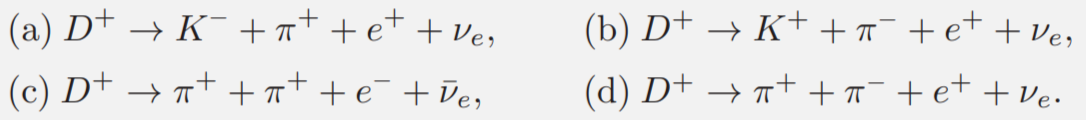
\includegraphics[width = .9\textwidth]{6.8.png}
\caption{Problem 6.8}
\label{fig: 6.8}
\end{figure}



\subsection*{Problem 4 (6.9)}
\begin{mdframed}
Which of the following six decays are allowed in lowest-order weak interactions \cref{fig: 6.9}?
\end{mdframed}
\begin{figure}[h!]
\centering
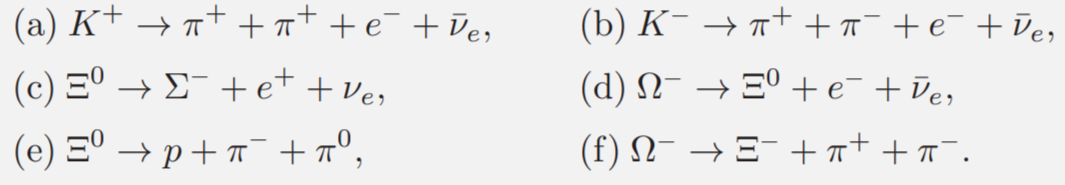
\includegraphics[width = .9\textwidth]{6.9.png}
\caption{Problem 6.9}
\label{fig: 6.9}
\end{figure}


\subsection*{Problem 5 (6.10)}
\begin{mdframed}
Use lepton universality and lepton–quark symmetry to estimate the branching ratios for the decays $b →  c + e^{-} + \bar{ν}_e$ (where the $b$ and $c$ quarks are bound in hadrons) and $τ^{-} →  e^{-} + \bar{ν}_e + ν_e$ . Ignore final states that are Cabibbo-suppressed relative to the lepton modes
\end{mdframed}

\end{document}